\documentclass[11pt]{article}
\usepackage[margin=1in,marginparwidth=0.78in,marginparsep=0.12in]{geometry}
\usepackage{amsmath,amssymb,amsthm}
\usepackage{tikz}
\usepackage[T1]{fontenc}
\usepackage{lmodern}
\usepackage{hyperref}
\hypersetup{pdftitle={Lie theory for posets and cones: a gentle introduction}}

\newtheorem{theorem}{Theorem}
\newtheorem{corollary}[theorem]{Corollary}
\theoremstyle{definition}
\newtheorem{fact}{Classical fact}
\newtheorem{example}{Example}
\newtheorem{question}{Question}
\newtheorem{conjecture}{Conjecture}
\theoremstyle{remark}
\newtheorem*{remark}{Remark}

\newcommand{\OP}{\mathcal O}
\newcommand{\Lin}{\operatorname{Lin}}
\newcommand{\Aut}{\operatorname{Aut}}
\newcommand{\Lie}{\operatorname{Lie}}
\newcommand{\PLie}{\mathsf{Lie}}
\newcommand{\sgn}{\operatorname{sgn}}
\newcommand{\Ind}{\operatorname{Ind}}
\newcommand{\Fix}{\operatorname{Fix}}
\newcommand{\lin}{\operatorname{lin}}
\newcommand{\Lune}{\mathrm{Lune}}
\newcommand{\src}[1]{\nolinkurl{#1}}
\emergencystretch=3em
\urlstyle{same}

% Status tags: a box in the margin, and a short inline label.
\newcommand{\tagbox}[1]{\leavevmode\marginpar{\raggedright\fbox{\parbox{0.66in}{\centering\scriptsize\sffamily #1}}}}
\newcommand{\PROVEN}{\tagbox{PROVEN\\AUDITED}}
\newcommand{\CITED}{\tagbox{CLASSICAL\\(CITED)}}
\newcommand{\COMPUTED}{\tagbox{COMPUTED}}
\newcommand{\CONJ}{\tagbox{CONJEC-\\TURED}}
\newcommand{\OPEN}{\tagbox{OPEN}}
\newcommand{\PARTIAL}{\tagbox{PROVEN\\NOT AUDITED}}
\newcommand{\KNOWN}{\tagbox{KNOWN\\(INSTANCE)}}
\newcommand{\REFUTED}{\tagbox{REFUTED\\AUDITED}}

\title{Lie theory for posets and cones:\\ a gentle introduction}
\author{}
\date{October 2026}

\begin{document}
\maketitle

\begin{abstract}
The free Lie algebra hides inside the partition lattice: the top homology of
the lattice of set partitions of $[n]$ is, up to a sign twist, the
multilinear part of the free Lie algebra on $n$ letters. This note explains,
with small pictures and examples, how that classical fact extends first to
finite posets and then to cones of real hyperplane arrangements and of
oriented matroids. It describes the fixed-point formula for the characters
that appear, says what is known about when those characters vanish, compares
the picture with six neighbouring theories, and says what the
generalization does and does not buy, including what it says about
promotion and cyclic sieving on linear extensions, and the one new
refined count it gives: a cyclic order polynomial whose $h$-vector counts
rotation classes of linear extensions by cyclic descents. The poset theorem is
now fully formalized in Lean. It is a summary. The proofs are in
the notes files named in the footnotes.
\end{abstract}

\section*{How to read this note}

Every stated result has a box in the margin and a footnote naming the
notes file (and section) it comes from. The boxes mean:
\begin{itemize}
\item \textsf{PROVEN / AUDITED}: the source note proves it, and an
  independent audit re-derived the proof (usually with its own code) and
  found that it holds. These are the only results stated as
  \emph{Theorems}. Some of them rest on a cited published theorem; the
  footnote says which.
\item \textsf{PROVEN / NOT AUDITED}: the source note gives a proof, but no
  independent audit has checked it yet.
\item \textsf{CLASSICAL (CITED)}: a published result, stated as background.
\item \textsf{KNOWN (INSTANCE)}: true and audited here, but it is a special
  case of a published theorem; the footnote names it.
\item \textsf{REFUTED / AUDITED}: a conjecture that a source note shows to
  be false by a counterexample, which an independent audit rebuilt and
  confirmed.
\item \textsf{COMPUTED}: checked by computer on the cases listed, not proved.
\item \textsf{CONJECTURED} and \textsf{OPEN}: what they say.
\end{itemize}
When we say a result was ``not found in the literature'', we mean that the
searches recorded in the notes did not find it. That is not a proof of
novelty.

\section{The classical story: Lie brackets in the partition lattice}

\subsection{Lie\texorpdfstring{$_n$}{n}}

Take the free Lie algebra on letters $x_1,\dots,x_n$ and keep the part that
uses each letter exactly once. Call it $\Lie_n$. It is spanned by bracketings
such as $[[x_2,x_3],x_1]$. The symmetric group $S_n$ acts by permuting the
letters, and $\dim\Lie_n=(n-1)!$: a basis is the left-normed brackets
$[\cdots[[x_1,x_{\sigma(2)}],x_{\sigma(3)}],\dots,x_{\sigma(n)}]$.

There is a second, very concrete model. Let $\gamma=(1\,2\,\cdots\,n)$, let
$\zeta$ be a primitive $n$th root of unity, and put
\[
e_\zeta=\frac1n\sum_{j=0}^{n-1}\zeta^{-j}\gamma^j\in\mathbb C[S_n].
\]
Think of a permutation as a word $w=w_1w_2\cdots w_n$. Right multiplication
by $\gamma$ rotates the word, and $w\gamma e_\zeta=\zeta\,we_\zeta$. So
$we_\zeta$ depends, up to a root of unity, only on the necklace (rotation
class) of $w$.

\begin{fact}[Klyachko]\CITED
$\Lie_n\cong\mathbb C[S_n]e_\zeta\cong\Ind_{C_n}^{S_n}\zeta$ as
$S_n$-modules.\footnote{As cited in \src{notes/poset_jks_research_note.tex},
\S3.1 and \src{notes/poset_jks_theorem.tex}, Cor.~3.16(a).}
\end{fact}

\subsection{The partition lattice}

Let $\Pi_n$ be the set partitions of $[n]$, ordered by refinement. The proper
part $\overline{\Pi_n}$ removes the bottom (all singletons) and the top (one
block). Figure~\ref{fig:pi3} shows $\Pi_3$: its proper part is three points,
so its reduced homology is $\widetilde H_0$, of dimension $2=(3-1)!$.

\begin{figure}[ht]
\centering
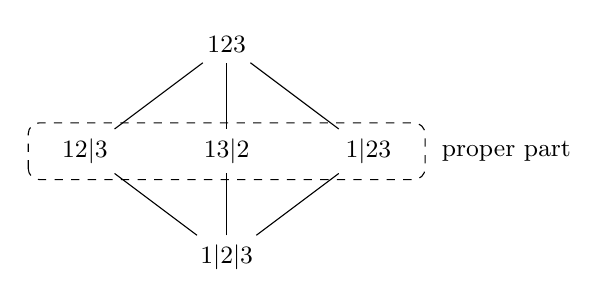
\begin{tikzpicture}[scale=0.9,every node/.style={font=\small}]
\node (b) at (0,0) {$1|2|3$};
\node (a1) at (-2,1.5) {$12|3$};
\node (a2) at (0,1.5) {$13|2$};
\node (a3) at (2,1.5) {$1|23$};
\node (t) at (0,3) {$123$};
\foreach \x in {a1,a2,a3} {\draw (b)--(\x); \draw (\x)--(t);}
\draw[dashed,rounded corners] (-2.8,1.1) rectangle (2.8,1.9);
\node[right] at (2.9,1.5) {proper part};
\end{tikzpicture}
\caption{$\Pi_3$. The proper part is three points, a wedge of two
$0$-spheres.}\label{fig:pi3}
\end{figure}

\begin{fact}[Joyal, Klyachko, Stanley; Hanlon]\CITED
$\overline{\Pi_n}$ has the homotopy type of a wedge of $(n-1)!$ spheres of
dimension $n-3$, and
\[
\widetilde H_{n-3}(\overline{\Pi_n};\mathbb C)\cong\sgn\otimes\Lie_n
\qquad\text{as $S_n$-modules.}
\]
Hanlon and Stanley computed the character through fixed points: for $g$ with
$k$ cycles all of length $d$,
$\mu(\Pi_n^g)=(-1)^{k-1}\mu(d)\,d^{k-1}(k-1)!$, and $\mu(\Pi_n^g)=0$ for every
other $g\ne1$.\footnote{\src{notes/poset_jks_theorem.tex}, Cor.~3.16(a);
Hanlon's method as read in \src{notes/novelty_search_2.md}, \S2.1.}
\end{fact}

Here $\Pi_n^g$ is the sublattice of partitions fixed by $g$, and $\mu$ is its
M\"obius number $\mu(\hat0,\hat1)$. The reason fixed points appear is the
first of the three ideas this note is organized around.

\medskip
\noindent\fbox{\parbox{0.96\linewidth}{\textbf{Idea 1 (characters are
M\"obius numbers of fixed lattices).} If the homology of a poset is
concentrated in one degree, the Hopf trace formula and P.~Hall's theorem
turn the trace of a symmetry $g$ on that homology into $\pm\mu$ of the
subposet of $g$-fixed elements. Computing a character becomes computing a
M\"obius number.}}

\section{Posets}

\subsection{Order-preserving partitions and linear extensions}

Now replace the $n$ unrelated letters by a finite poset $P$ on $[n]$. A set
partition $\pi$ is \emph{order-preserving} if collapsing each block to a point
leaves a directed graph without cycles. These partitions form a lattice
$\OP(P)$. For the antichain nothing is forbidden and $\OP(P)=\Pi_n$. For the
chain $1<2<3$ the partition $13|2$ is forbidden, because $1<2<3$ would become
a cycle between the blocks $\{1,3\}$ and $\{2\}$.

A \emph{linear extension} of $P$ is a word $w$ in which $i$ comes before $j$
whenever $i<_Pj$. Write $\Lin(P)$ for the set of them, and $e_C(P)$ for the
number of rotation classes of words that contain at least one linear
extension. If $P$ is connected, no two linear extensions are rotations of
each other, so $e_C(P)=|\Lin(P)|$.

\begin{fact}[Jen\v{c}a--Sarkoci]\CITED
For $n\ge3$, the proper part of $\OP(P)$ is homotopy equivalent to a wedge of
$e_C(P)$ spheres of dimension $n-3$.\footnote{Cited as input~(A) in
\src{notes/poset_jks_theorem.tex}, \S2; the statement was checked against
the source in \src{notes/citation_check.md}, \S2.}
\end{fact}

Figure~\ref{fig:n3} lists the five posets on three points.

\begin{figure}[ht]
\centering
\tikzset{dot/.style={circle,fill,inner sep=1.2pt},pl/.style={font=\scriptsize}}
\begin{tabular}{lccccc}
 &
\begin{tikzpicture}[baseline=0]
\node[dot,label={[pl]below:$1$}] at (0,0) {}; \node[dot,label={[pl]below:$2$}] at (0.45,0) {}; \node[dot,label={[pl]below:$3$}] at (0.9,0) {};
\end{tikzpicture}
&
\begin{tikzpicture}[baseline=0]
\node[dot,label={[pl]below:$1$}] (x) at (0,0) {}; \node[dot,label={[pl]above:$2$}] (y) at (0,0.8) {}; \node[dot,label={[pl]below:$3$}] at (0.5,0) {};
\draw (x)--(y);
\end{tikzpicture}
&
\begin{tikzpicture}[baseline=0]
\node[dot,label={[pl]below:$1$}] (x) at (0.3,0) {}; \node[dot,label={[pl]above:$2$}] (y) at (0,0.8) {}; \node[dot,label={[pl]above:$3$}] (z) at (0.6,0.8) {};
\draw (x)--(y); \draw (x)--(z);
\end{tikzpicture}
&
\begin{tikzpicture}[baseline=0]
\node[dot,label={[pl]below:$1$}] (x) at (0,0) {}; \node[dot,label={[pl]below:$2$}] (y) at (0.6,0) {}; \node[dot,label={[pl]above:$3$}] (z) at (0.3,0.8) {};
\draw (x)--(z); \draw (y)--(z);
\end{tikzpicture}
&
\begin{tikzpicture}[baseline=0]
\node[dot,label={[pl]right:$1$}] (x) at (0,0) {}; \node[dot,label={[pl]right:$2$}] (y) at (0,0.45) {}; \node[dot,label={[pl]right:$3$}] (z) at (0,0.9) {};
\draw (x)--(y)--(z);
\end{tikzpicture}
\\[2pt]
 & antichain & $1<2$, $3$ & $1<2,\ 1<3$ & $1<3,\ 2<3$ & chain\\\hline
$|\Lin(P)|$ & 6 & 3 & 2 & 2 & 1\\
$|\OP(P)|$ & 5 & 5 & 5 & 5 & 4\\
$e_C(P)=\dim\widetilde H_0$ & 2 & 2 & 2 & 2 & 1
\end{tabular}
\caption{The posets on three points, by direct enumeration. For the second
poset the three linear extensions $123,312,132$ form two rotation classes,
$\{123,312\}$ and $\{132\}$. For the chain, $\OP(P)$ is the Boolean lattice
$\{1|2|3,\ 12|3,\ 1|23,\ 123\}$.}\label{fig:n3}
\end{figure}

\subsection{The poset Lie module}

Define
\[
\PLie(P)=\operatorname{span}\{we_\zeta: w\in\Lin(P)\}\subseteq\mathbb C[S_n].
\]
Its dimension is $e_C(P)$, and the automorphism group $\Aut(P)$ acts on it by
relabelling letters. For the antichain it is all of $\mathbb C[S_n]e_\zeta$,
which is $\Lie_n$. Let $H_P=\widetilde H_{n-3}(\overline{\OP(P)};\mathbb C)$.

\begin{theorem}[poset JKS]\label{thm:posetjks}\PROVEN
Let $P$ be a finite poset on $n\ge3$ points. Then
$H_P\cong\sgn\otimes\PLie(P)$ as $\Aut(P)$-modules. Equivalently, for every
$g\in\Aut(P)$,
\[
(-1)^{n-3}\mu\bigl(\OP(P)^g\bigr)=\sgn(g)\sum_{C\,:\,gC=C}\zeta^{r_g(C)},
\]
where $C$ runs over the rotation classes meeting $\Lin(P)$ that $g$ maps to
themselves, and $r_g(C)$ is the rotation by which $g$ acts on $C$. Moreover
both sides equal $\sgn(g)\,\mu(o)\sum_{x\in F(P,g)}e_C(P|_{B_0(x)})$, where $o$
is the order of $g$, $\mu(o)$ is the number-theoretic M\"obius function, and
$F(P,g)$ is the set of partitions into $o$ blocks, each a union of connected
components, that $g$ permutes cyclically ($B_0(x)$ is any block).%
\footnote{\src{notes/poset_jks_theorem.tex}, \S3, Theorem~3.1. Two
independent proofs, both audited in
\src{notes/audit_character_identity_proof.md} (``proof holds''). The proof
uses Jen\v{c}a--Sarkoci, P.~Hall's theorem and the Hopf trace formula, all
cited; all three, and the theorem itself, are now proved in Lean
(\S\ref{sec:lean}). The isomorphism is abstract (equal characters); an explicit
choice-free isomorphism is in \S6 of the same file.}
\end{theorem}

For the antichain this is the classical JKS theorem. The right-hand side
of the character identity has a plain meaning: it is a sum over the rotation
classes of linear extensions that $g$ fixes, each weighted by a root of unity.
At $g=1$ it is the count $e_C(P)$, and the identity becomes
$\mu(\OP(P))=(-1)^{n-1}e_C(P)$. That count also has a proof with no topology
at all: one application of Weisner's theorem and Jen\v{c}a--Sarkoci's
recursion for $e_C$.\footnote{\src{notes/mu_op_elementary.md}, Theorem~A
(Proof~W), audited in \src{notes/audit_mu_op_elementary.md}: both proofs
hold and are homology-free.}\PROVEN

\begin{corollary}\PROVEN
If $P$ is connected and $n\ge3$, then $\mu(\OP(P)^g)=0$ for every $g\ne1$, and
$H_P$ is a free $\Aut(P)$-module of rank $|\Lin(P)|/|\Aut(P)|$.\footnote{%
\src{notes/poset_jks_theorem.tex}, Cor.~3.15; audited in
\src{notes/audit_character_identity_proof.md}, II7.}
\end{corollary}

So roots of unity appear only when $g$ permutes connected components freely.

More is true at the level of spaces. For connected $P$, the order complex of
the proper part of $\OP(P)$ is a wedge of $e_C(P)=|\Lin(P)|$ spheres that $\Aut(P)$
permutes freely, up to $\Aut(P)$-equivariant homotopy, so $H_P$ is free even
over $\mathbb Z[\Aut(P)]$.\footnote{%
\src{notes/theorem_e_equivariant_wedge.md}, Theorem~E and \S2.5; audited in
\src{notes/audit_theorem_e.md} (it holds). For the claw (one point below all
the others), where $\OP(P)=\Pi_n$, this is the known splitting of the
partition complex under $S_{n-1}$ (Arone; Arone--Brantner; Donau); for other
connected $P$ we did not find it (\src{notes/prior_art_theorem_e.md}).}\PROVEN

\begin{example}[a fixed-point computation]\label{ex:fixed}
Let $P$ be two disjoint chains $1<2$ and $3<4$, and let $g=(13)(24)$ swap
them. The linear extensions are the six shuffles of $12$ and $34$. The words
$1234$ and $3412$ are rotations of each other, and the other four lie in four
further classes, so $e_C(P)=5$ and $\dim H_P=5$.

\emph{Lie side.} Only the class $\{1234,3412\}$ is fixed by $g$: $g$ sends
$1234$ to $3412$, which is $1234$ rotated by two places. With $\zeta=i$ the
phase is $\zeta^2=-1$. So the trace of $g$ on $\PLie(P)$ is $-1$.

\emph{M\"obius side.} The $g$-fixed order-preserving partitions are drawn in
Figure~\ref{fig:fixed}. Counting upwards, $\mu$ is $-1$ on the three atoms,
$+1$ on $13|24$ and $+1$ on the top. So $(-1)^{4-3}\mu(\OP(P)^g)=-1$, and
$\sgn(g)=+1$. The two sides agree. The closed formula gives the same number:
$o=2$, $\mu(2)=-1$, $F(P,g)=\{12|34\}$, and $e_C$ of a $2$-chain is $1$.

\emph{Why it works (Weisner).} The orbit partition of $g$ is
$O_g=13|24$. Weisner's theorem says that the M\"obius numbers $\mu(\hat0,x)$
of the $x$ with $x\vee O_g=\hat1$ sum to zero. Here those $x$ are $12|34$ and
$\hat1$, so $\mu(\hat0,\hat1)=-\mu(\hat0,12|34)=1$. The general proof is this
step plus a M\"obius inversion.\footnote{\src{notes/poset_jks_theorem.tex},
\S3.2, Prop.~3.11 and Lemma~3.8 (Weisner). The computation in this example was done by
hand and by direct enumeration.}
\end{example}

\begin{figure}[ht]
\centering
\begin{tikzpicture}[scale=0.95,every node/.style={font=\small}]
\node (b) at (0,0) {$1|2|3|4$};
\node (a) at (-2.6,1.4) {$13|2|4$};
\node (c) at (0,1.4) {$1|24|3$};
\node (d) at (2.8,1.4) {$12|34$};
\node (e) at (-1.3,2.8) {$13|24$};
\node (t) at (0.6,4.2) {$1234$};
\draw (b)--(a); \draw (b)--(c); \draw (b)--(d);
\draw (a)--(e); \draw (c)--(e); \draw (e)--(t); \draw (d)--(t);
\node[gray] at (-3.8,1.4) {$-1$}; \node[gray] at (1.05,1.4) {$-1$}; \node[gray] at (3.95,1.4) {$-1$};
\node[gray] at (-2.3,2.8) {$+1$}; \node[gray] at (1.6,4.2) {$+1$}; \node[gray] at (1.0,0) {$+1$};
\end{tikzpicture}
\caption{The lattice $\OP(P)^g$ for $P=\{1<2\}\sqcup\{3<4\}$ and $g=(13)(24)$,
with $\mu(\hat0,x)$ in grey.}\label{fig:fixed}
\end{figure}

\begin{remark}
The first proposed route to Theorem~\ref{thm:posetjks} was to show that one
fixed classical JKS isomorphism maps $H_P$ onto $\PLie(P)$. That is false
already for a chain and its reverse: they have the same $\OP$, but different
spans $\mathbb C\,we_\zeta$.\footnote{\src{notes/poset_jks_theorem.tex}, \S4,
Prop.~4.2; audited in \src{notes/audit_literature_novelty_jks_maps.md}.}%
\PROVEN{} The correct restricted statement replaces $\mathbb C[S_n]e_\zeta$
by $\mathbb C[S_n]$ modulo shuffles. That leads to the second idea.
\end{remark}

\section{Geometry: chambers, cones and lunes}

\subsection{The braid arrangement}

The braid arrangement is the set of hyperplanes $x_i=x_j$ in $\mathbb R^n$.
Its chambers (the regions where all coordinates differ) are the
permutations: the chamber of $w$ is $x_{w_1}<x_{w_2}<\cdots<x_{w_n}$. A poset
cuts out the \emph{order cone}
\[
C_P=\{x\in\mathbb R^n: x_i\le x_j\text{ whenever }i<_Pj\},
\]
and the chambers inside $C_P$ are exactly the linear extensions of $P$.
Figure~\ref{fig:A2} shows $n=3$, after quotienting by the line
$x_1=x_2=x_3$: three lines, six chambers.

\begin{figure}[ht]
\centering
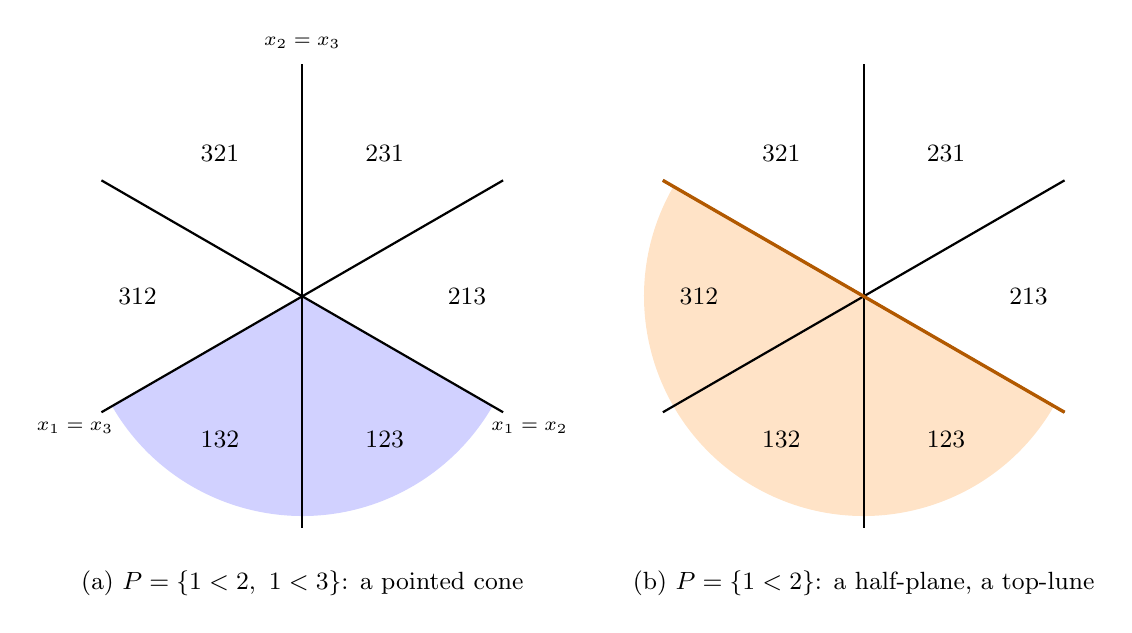
\begin{tikzpicture}[scale=1.55,every node/.style={font=\small}]
\begin{scope}
\fill[blue!18] (0,0) -- (210:1.8) arc (210:330:1.8) -- cycle;
\foreach \a in {90,210,330} {\draw[thick] (\a:1.9)--(\a+180:1.9);}
\foreach \a/\w in {300/123,240/132,180/312,120/321,60/231,0/213} {\node at (\a:1.35) {$\w$};}
\node[font=\scriptsize] at (90:2.08) {$x_2=x_3$};
\node[font=\scriptsize] at (330:2.15) {$x_1=x_2$};
\node[font=\scriptsize] at (210:2.15) {$x_1=x_3$};
\node at (0,-2.35) {(a) $P=\{1<2,\ 1<3\}$: a pointed cone};
\end{scope}
\begin{scope}[xshift=4.6cm]
\fill[orange!22] (0,0) -- (150:1.8) arc (150:330:1.8) -- cycle;
\foreach \a in {90,210,330} {\draw[thick] (\a:1.9)--(\a+180:1.9);}
\draw[very thick,orange!70!black] (150:1.9)--(330:1.9);
\foreach \a/\w in {300/123,240/132,180/312,120/321,60/231,0/213} {\node at (\a:1.35) {$\w$};}
\node at (0,-2.35) {(b) $P=\{1<2\}$: a half-plane, a top-lune};
\end{scope}
\end{tikzpicture}
\caption{The braid arrangement $A_2$. (a) The order cone of $1<2,\ 1<3$
contains the chambers $123$ and $132$. Its faces span three lines, so its
support lattice has three middle elements and $m(V)=2$. (b) The order cone of
$1<2$ is a half-plane containing $123,132,312$. It contains the line
$x_1=x_2$ (its lineality space), and it is itself a top-lune.}\label{fig:A2}
\end{figure}

Faces of the arrangement inside $C_P$ correspond to order-preserving maps
$P\to[k]$ onto chains, and the linear span of a face is recorded by the
partition into fibres. In this way the lattice of spans of faces of $C_P$ is
$\OP(P)$, turned upside down.\footnote{\src{notes/cone_lune_lie_theory.md},
\S2, Prop.~2.1 (audited in \src{notes/audit_cone_lune_lie_theory.md}), and
\src{notes/general_theory.md}, \S1.3, Cor.~1.4 (audited in
\src{notes/audit_general_theory_cones.md}).}\PROVEN

\subsection{Any arrangement, any cone}

Let $\mathcal A$ be a finite central arrangement of hyperplanes in
$\mathbb R^d$, essential (the hyperplanes meet only in $0$). A
\emph{top-cone} $V$ is a nonempty set of chambers obtained by choosing a side
of some of the hyperplanes. Its \emph{support lattice} $\Lambda(V)$ is the set
of subspaces spanned by faces of $\mathcal A$ that lie in the closed cone
$|V|$, ordered by inclusion. Put $m(V)=(-1)^d\mu(\Lambda(V))$. The
\emph{lineality space} $\lin V=|V|\cap-|V|$ is the largest subspace inside the
cone. The cone is \emph{pointed} if $\lin V=0$.

\begin{theorem}[cone wedge theorem]\label{thm:wedge}\PROVEN
For every top-cone $V$ of a finite real central essential arrangement of
rank $d$, the proper part of $\Lambda(V)$ is homotopy equivalent to a wedge
of $m(V)$ spheres of dimension $d-2$.\footnote{\src{notes/general_theory.md},
\S1.1, Theorem~1; audited in \src{notes/audit_general_theory_cones.md}
(holds; the cited fibre theorem of Bj\"orner--Wachs--Welker can be removed,
Prop.~A there). We did not find it in the literature
(\src{notes/novelty_general_theory.md}, \S2).}
\end{theorem}

For the braid arrangement and $V=C_P$ this is the Jen\v{c}a--Sarkoci theorem,
with a new proof, and $m(C_P)=e_C(P)$. For $V$ = all chambers it is Folkman's
theorem for geometric lattices.

\begin{theorem}[Zaslavsky for cones]\PROVEN
$\#V=\sum_X m(V_X)$, where $X$ runs over the flats contained in $\lin V$ and
$V_X$ is the image of $V$ in $\mathbb R^d/X$. If $V$ is pointed,
$\#V=m(V)$.\footnote{\src{notes/general_theory.md}, \S1.2, Theorem~2;
audited in \src{notes/audit_general_theory_cones.md}. It is a short
specialization of Zaslavsky's 1977 dissection theorem
(\src{notes/novelty_general_theory.md}, \S3).}
\end{theorem}

In Figure~\ref{fig:A2}(b), $\#V=3$, $m(V)=2$, and the line $x_1=x_2$
contributes $1$. In the braid case the theorem reads
$|\Lin(P)|=\sum_\sigma\prod_{B\in\sigma}e_C(P|_B)$, a sum over partitions
$\sigma$ of the components of $P$.

\subsection{Lie elements are what lunes cannot see}

A \emph{top-lune} is the set of chambers lying on prescribed sides of all the
hyperplanes through some fixed flat. In the braid arrangement the top-lunes
are the sets of shuffles of a few words, for example $\{123,132,312\}$, the
shuffles of $12$ and $3$. Let $\Gamma$ be the space spanned by the chambers,
and let $\Lune\subseteq\Gamma$ be spanned by the sums over top-lunes with more
than one chamber. The Lie elements of the arrangement, in the sense of
Aguiar--Mahajan, are the vectors orthogonal to $\Lune$. For the braid
arrangement $\Lune$ is the span of the proper shuffles, and its orthogonal is
$\Lie_n$ (Ree).\footnote{Aguiar--Mahajan, \emph{Topics in Hyperplane
Arrangements}, Lemmas 10.7--10.8, as read in
\src{notes/literature_novelty_jks_maps.md}, \S4.2, and
\src{notes/cone_lune_lie_theory.md}, \S1.}\CITED

\medskip
\noindent\fbox{\parbox{0.96\linewidth}{\textbf{Idea 2 (chambers modulo
lunes).} The Lie module of a cone is the span of its chambers, modulo the
lunes. The top homology of the cone's support lattice is that module,
twisted by the determinant.}}

\begin{theorem}[cone JKS]\label{thm:G}\PROVEN
Let $V$ be a top-cone of a finite real central essential arrangement in
$\mathbb R^d$, $d\ge2$, and let $G$ be a finite group of linear maps
preserving $\mathcal A$. Write $\Gamma_V$ for the span of the chambers of $V$.
Then
\[
\widetilde H_{d-2}\bigl(\overline{\Lambda(V)};\mathbb C\bigr)\cong
\det\otimes\,(\Gamma_V+\Lune)/\Lune
\]
as modules over the stabilizer of $V$ in $G$. In particular $m(V)$ equals
$\dim\Gamma_V/(\Gamma_V\cap\Lune)$.\footnote{Proved as Theorem~C in
\src{notes/audit_general_theory_cones.md}, \S C, given a theorem of Brown on
left regular bands (cited, read in the source); restated as Theorem~G$^*$
in \src{notes/general_theory.md}, \S1.5. Independently audited in
\src{notes/audit_theorem_c.md} (holds with fixes to proofs; no conclusion
changes). For $V$ = all chambers it is known (Aguiar--Mahajan, \emph{Topics},
Thm.~14.32); for proper cones we did not find it
(\src{notes/novelty_general_theory.md}, \S5).}
\end{theorem}

For $C_P$ the determinant is $\sgn$, and Theorem~\ref{thm:G} says
$H_P\otimes\sgn\cong\mathbb C[\Lin P]/(\text{lunes inside }C_P)$. That is the
poset theorem in a form that names an explicit basis: the splitting cycles of
the linear extensions.\footnote{\src{notes/poset_jks_theorem.tex}, \S5,
Theorem~5.3(d), which is proved there given a cited theorem of Wachs; by
Theorem~\ref{thm:G} it also holds given Brown
(\src{notes/general_theory.md}, \S1.5).}
In Figure~\ref{fig:A2}(b), three chambers modulo one lune leave a
two-dimensional space, and $m(V)=2$. A pointed cone contains no lune with
more than one chamber, and its chambers are independent modulo lunes.

\subsection{Oriented matroids}

Nothing above needs coordinates. An oriented matroid keeps only the sign
vectors of the faces, and some oriented matroids come from no real
arrangement. The role of a top-cone is played by a $T$-convex set of topes.

\begin{theorem}\PROVEN
For every simple oriented matroid of rank $r$ and every nonempty $T$-convex
set $V$ of topes: the proper part of $\Lambda(V)$ is a wedge of $m(V)$ spheres
of dimension $r-2$; the Zaslavsky count holds; and the top homology is
$\det\otimes(\Gamma_V+\Lune)/\Lune$ as a module over the stabilizer of $V$,
given Brown. Realizability is not used.\footnote{%
\src{notes/oriented_matroid_cones.md}, Verdict table, Theorems 1-OM, 2-OM and
C-OM; audited in \src{notes/audit_oriented_matroid_cones.md}: every claim
holds, with one wrong attribution fixed. For $r\ge5$ the homotopy form uses
shellability of the tope complex (cited).}
\end{theorem}

\section{Characters: the fixed-point formula}

Let $g$ be a linear map of finite order with $g\mathcal A=\mathcal A$ and
$gV=V$, for instance an automorphism of $P$ acting on $C_P$. By Idea~1 its
character on the top homology is
\[
\chi_V(g)=(-1)^d\det(g)\,\mu\bigl(\Lambda(V)^g\bigr),
\]
where $\Lambda(V)^g$ is the lattice of $g$-stable spans. In the braid case
this is the left side of Theorem~\ref{thm:posetjks}, multiplied by
$\sgn(g)$.

\begin{theorem}[equivariant cone Zaslavsky]\label{thm:EZ}\PROVEN
The number of chambers of $V$ fixed by $g$ is
\[
\#V^g=\sum_{X}\chi_{V_X}(\bar g),
\]
the sum over the $g$-stable flats $X\subseteq\lin V$, where $\bar g$ is the
map induced on $\mathbb R^d/X$. Inverting this over the lattice of $g$-stable
flats gives a closed formula for $\chi_V(g)$ in terms of chambers fixed by
$g$, which can be counted on the fixed space $\Fix(g)$.\footnote{%
\src{notes/fixed_point_formula.md}, Verdict table, rows EZ and CF; audited
in \src{notes/audit_fixed_point_formula.md} (holds, with fixes). For $V$ =
all chambers both are known in substance (Moseley; Sundaram--Welker); for
proper cones we did not find them (\src{notes/novelty_fixed_point_formula.md},
\S\S2--3).}
\end{theorem}

At $g=1$ this is the cone Zaslavsky theorem. On a pointed cone it says
$\chi_V(g)=\#V^g$. If $\mathcal A$ is the reflection arrangement of a
reflection group $W$ and $1\ne g\in W$, then $g$ fixes no chamber, so the top
homology of a pointed cone is a free module over the stabilizer of $V$ in
$W$.\footnote{\src{notes/fixed_point_formula.md}, Cor.~P; audited in
\src{notes/audit_fixed_point_formula.md}.}\PROVEN{} This is the analogue of
the connected-poset corollary. For the braid arrangement the formula of
Theorem~\ref{thm:EZ} agrees with the closed formula of
Theorem~\ref{thm:posetjks}.

\section{When does the character vanish?}

\medskip
\noindent\fbox{\parbox{0.96\linewidth}{\textbf{Idea 3 (transverse flats).}
Whether $\chi_V(g)$ can be nonzero is decided by the $g$-stable flats $X$
that meet $\Fix(g)$ only in $0$ and are transverse to it (no hyperplane
contains $X+\Fix(g)$), and by the M\"obius numbers of their fixed lattices.}}

\medskip
Write $Z^*(V,g)$ for the $g$-stable flats $X\subseteq\lin V$ with
$X\cap\Fix(g)=0$ such that no hyperplane of $\mathcal A$ contains
$X+\Fix(g)$, and $Z^*(g)$ for the same set with $V$ = all chambers.

\begin{theorem}[Formula Z and the some-cone criterion]\PROVEN
\[
\chi_V(g)=\sum_{X\in Z^*(V,g)}\mu_{L(\mathcal A)^g}(0,X)\,m_X(V),
\qquad m_X(V)\ge1,
\]
where $L(\mathcal A)^g$ is the lattice of $g$-stable flats and $m_X(V)$ is
the multiplicity of a smaller cone inside $\Fix(g)$. Consequently
$\chi_V(g)\ne0$ for some $g$-stable top-cone $V$ if and only if some
$X\in Z^*(g)$ has $\mu(0,X)\ne0$, and then a top-lune witnesses it.%
\footnote{\src{notes/vanishing_criterion.md}, Verdict table, rows Z and S;
audited twice, in \src{notes/audit_vanishing_criterion.md} and
\src{notes/audit2_vanishing_criterion.md} (both: holds). We did not find
either statement for proper cones
(\src{notes/prior_art_vanishing_criterion.md}, \S\S2--3).}
\end{theorem}

\begin{theorem}[type A, all of $\pm S_n$]\PROVEN
On the braid arrangement in $\mathbb R^n$ ($n\ge3$), let $g=\pm w$ with
$w\in S_n$. Some $g$-stable cone has $\chi\ne0$ if and only if $\langle
g\rangle$ acts freely on $\{\pm e_1,\dots,\pm e_n\}$ and $\mu(\operatorname{ord}
g)\ne0$. For $+w$ this is the classical rule ``all cycles of one length $o$,
with $\mu(o)\ne0$''. For $-w$ it says that the cycle lengths of $w$ lie in
$\{m,2m\}$ for one odd squarefree $m$.\footnote{%
\src{notes/vanishing_criterion.md}, row A and \S4; audited in both audits
named above.}
\end{theorem}

The map $-w$ preserves an order cone $C_P$ exactly when $w$ is an
anti-automorphism of $P$ (it reverses every relation), so the second half is
about anti-automorphisms of posets. Since $\OP(P)=\OP(P^{\mathrm{op}})$,
they act on $\OP(P)$ too.\footnote{\src{notes/per_cone_vanishing.md}, \S3;
\src{notes/poset_jks_theorem.tex}, Lemma~4.1.} Already for
$n\le7$ there are nine classes $-w$ that are nonzero on some cone but zero on
all chambers, for example $-(2,1)$.\footnote{%
\src{notes/prior_art_vanishing_criterion.md}, \S4.}\COMPUTED{} The rule for
$-w$ is invisible if one looks only at all chambers.

\paragraph{Per cone.} Formula Z can cancel: nonzero terms of opposite sign can
add to zero. In type A this is completely understood.

\begin{theorem}[type A, every cone]\label{thm:TA}\PROVEN
Let $\tau$ be an anti-automorphism of $P$ ($n\ge3$). Call a point odd if it lies on an odd cycle of $\tau$. Then
$\chi_{C_P}(-\tau)\ne0$ if and only if
\begin{enumerate}
\item[(1)] the cycle lengths of $\tau$ lie in $\{m,2m\}$ for one odd
  squarefree $m$;
\item[(2)] the $\langle\tau\rangle$-orbit of every component $K$ of $P$ has
  length $m$ or $2m$;
\item[(3)] for every component $K$, the set $K\cup\tau^mK$ contains at most
  one odd point;
\item[(4)] if $\tau$ has both odd and even cycles, some odd cycle of $\tau$
  does not consist of isolated points of $P$.
\end{enumerate}
There is a positive closed formula for $|\chi_{C_P}(-\tau)|$. With Theorem~\ref{thm:posetjks} for $+w$,
this decides vanishing for every element of $\pm S_n$ on every cone of the
braid arrangement.\footnote{\src{notes/per_cone_vanishing.md}, \S3, Theorem~TA
and row TA$\pm$. Audited in \src{notes/audit_per_cone_vanishing.md}:
``holds with fixes''; the fixes are to proofs and do not change a result,
and they have been applied to the source note. A search found no statement
of Theorem~TA in the literature
(\src{notes/prior_art_per_cone_vanishing.md}, Verdict table).}
\end{theorem}

One ingredient is a small fact about linear extensions: an anti-automorphism
$t$ of a poset has a linear extension $w$ with $t(w_i)=w_{n+1-i}$ for all $i$
(a ``$t$-palindromic'' extension) if and only if $t^2=1$ and $t$ has at most
one fixed point.\footnote{\src{notes/per_cone_vanishing.md}, \S2, Lemma~Pal;
audited in \src{notes/audit_per_cone_vanishing.md} (holds; checked on all
$6{,}847$ anti-automorphisms with $n\le7$).}\PROVEN{} These palindromic
extensions are the chambers that $-t$ fixes. The lemma is known in
substance: after relabelling, the palindromic extensions are the type-B
linear extensions of a $B_n$ poset (Chow; Reiner for signed
posets).\footnote{\src{notes/prior_art_per_cone_vanishing.md}, Verdict
table, rows Lemma Pal. The exact ``iff'' form was not found stated.}

\paragraph{What is open.}
\begin{itemize}
\item \OPEN An exact per-cone vanishing criterion beyond type A: for $B_n$
  ($n\ge5$), $D_n$, $H_3$, $H_4$, $F_4$ and general arrangements. Off the
  Coxeter examples, cancellation is common.\footnote{Rows PC$'$ and PC$''$ of
  \src{notes/vanishing_criterion.md}, and rows B, D, H, F of
  \src{notes/per_cone_vanishing.md}.}
\item \CONJ The Crapo-type converse on all chambers. By Crapo's
  complementation theorem, if the
  interval $[0,X]$ of the fixed lattice has an element with no complement,
  then $\mu(0,X)=0$. On all chambers, the converse held for all 191 flats
  $X\in Z^*(g)$ tested.%
  \footnote{\src{notes/vanishing_criterion.md}, row CR.}
\item \REFUTED The Crapo-type converse on cones (Conjecture CR$_V$):
  $\chi_V(g)=0$ if and only if $\Lambda(V)^g$ has an element
  with no complement. It is false in rank~$4$. No counterexample was found
  on the first $18{,}750$ pairs $(V,g)$ tested.\footnote{\src{notes/per_cone_vanishing.md}, row
  CR$_V$ and \S4. A search found no statement of the conjecture. The
  converse is false for general finite lattices, and it is known for finite
  modular lattices (Knop), a class that does not contain the lattices
  $\Lambda(V)^g$ in general (\src{notes/prior_art_per_cone_vanishing.md},
  Verdict table).} A later note gives a counterexample in rank~$4$: a
  $12$-hyperplane arrangement in $\mathbb R^4$ where a cancellation $1-1=0$
  in Formula~Z sits on a $9$-element lattice in which every element has a
  complement.\footnote{%
  \src{notes/conjecture_cr_v.md}, \S0 and Verdict table. Independently
  audited in \src{notes/audit_conjecture_cr_v.md}: the refutation holds;
  the counterexample was rebuilt from the definitions, and $\chi_V(g)=0$ was
  confirmed in four independent ways.}
  So the converse is false in general, but true for posets: on every cone
  of the braid arrangement (every poset $P$, every automorphism or
  anti-automorphism), $\chi_V(g)=0$ forces an explicit element of
  $\Lambda(V)^g$ with no complement, in every rank.\footnote{%
  \src{notes/cr_v_type_a.md}, Theorem TA-CR; independently audited in
  \src{notes/audit_cr_v_type_a.md} (it holds). The ``if'' direction is
  Crapo's corollary. A search found the ``only if'' direction
  only for the antichain with an automorphism (Stanley 1982, with Hanlon
  1981), not for general posets
  (\src{notes/prior_art_cr_v_type_a.md}).}
  Moreover, every such zero has an explicit, uniform witness with no
  complement, given by one of two formulas.\footnote{%
  \src{notes/observation_cc.md}, Theorem~CC and Cor.~U; independently
  audited in \src{notes/audit_observation_cc.md} (it holds).}
\item \PROVEN The converse does hold in rank at most~$3$ and for pointed
  cones in every rank: there $\chi_V(g)=0$ forces an element of
  $\Lambda(V)^g$ with no complement. In every rank, each zero in which a
  hyperplane contains $\lin V+\Fix g$ (a ``Cor.~V'' zero) comes with such an
  element, explicitly.\footnote{\src{notes/conjecture_cr_v.md}, Theorems~3, P
  and~Q; audited in \src{notes/audit_conjecture_cr_v.md} (all three
  hold).}
\item \PROVEN In type A, whether $\chi_V(g)=0$ depends only on
  $(\lin V,g)$.\footnote{\src{notes/per_cone_vanishing.md}, row TA-L
  (Cor.~3.5); audited in \src{notes/audit_per_cone_vanishing.md}.}
\item \COMPUTED In general it does not: generic arrangements of four planes
  in $\mathbb R^3$ already give counterexamples.\footnote{%
  \src{notes/per_cone_vanishing.md}, row L$'$ and \S4.}
\end{itemize}

\section{Neighbouring theories}

Each paragraph names the analogy and where it stops. Several primary sources
could not be opened, and the notes record them as \emph{not accessible};
statements about them below come from secondary accounts.

\paragraph{Orlik--Solomon algebras and Lehrer--Solomon.} The Orlik--Solomon
algebra is the cohomology of the complement of the complexified arrangement.
Lehrer--Solomon describe the $S_n$-action on it as a sum of modules induced
from centralizers. On all chambers, the cone character $\chi$ is the top
Orlik--Solomon character twisted by $\det$ (Orlik--Solomon 1980,
Thm.~4.8).\footnote{\src{notes/prior_art_vanishing_criterion.md}, Verdict
table, \S0.3 and \S1; \src{notes/novelty_fixed_point_formula.md}, \S4.
Orlik--Solomon 1980, Thm.~4.8, was read in the source
(\src{notes/prior_art_vanishing_criterion.md}, \S1). Lehrer 1987 and
Lehrer--Solomon 1986 were read only through secondary accounts.} The
analogy stops at cones. That theory concerns the whole complement, so it
sees only all chambers. The cone theory decomposes the space spanned by
chambers instead. For all chambers that decomposition matches the cohomology
of a different space, Moseley's complement $M_3(\mathcal A)$ of the
codimension-three subspaces, and it differs from the Orlik--Solomon one by a
determinant twist on each summand. Nothing in those
accounts mentions fixed chambers, cones or lineality spaces.

\paragraph{Lie characters of Coxeter groups.} For a reflection group $W$,
the Lie module of the whole arrangement is a $W$-module, and Aguiar--Mahajan
prove a JKS theorem for every arrangement, with the twist carried by an
orientation space. This is the all-chambers case of Theorem~\ref{thm:G}.%
\footnote{\src{notes/novelty_general_theory.md}, \S5.} Bishop, Douglass,
Pfeiffer and R\"ohrle give a necessary support condition for the top
Orlik--Solomon component through cuspidal classes, for groups of rank at
most $8$ and for all chambers only.\footnote{%
\src{notes/prior_art_vanishing_criterion.md}, \S3.} The cone theory
adds proper cones and symmetries outside $W$, such as $-w$ in type A. The
type-A support rule does not generalize in the obvious way: Springer
regularity is neither necessary nor sufficient for being nonzero on some
cone. The Coxeter element of $B_3$ vanishes on every cone, and a reflection
of $B_2$ does not.\footnote{\src{notes/vanishing_criterion.md}, row R; proven
by hand given the some-cone criterion, audited in
\src{notes/audit_vanishing_criterion.md}.}\PROVEN

\paragraph{Aguiar--Mahajan: Hopf monoids, cones and lunes.} The vocabulary
here (Tits product, top-lunes, Lie elements as $\Lune^\perp$) is
Aguiar--Mahajan's. In the parts of their books that were read we found no
theory attached to a single cone, and one exercise needed correcting: an element is Lie iff its coefficient sum
vanishes on every \emph{non-pointed} top-cone, not every non-singleton
one.\footnote{\src{notes/cone_lune_lie_theory.md}, \S7, audited in
\src{notes/audit_cone_lune_lie_theory.md};
\src{notes/literature_novelty_jks_maps.md}, \S4.3.}\PROVEN{} The natural
first guess, the left regular band of faces of the cone acting on its own
chambers, gives zero for the chain, and on all proper order cones tested.
The right object is the ambient Lie module restricted to the cone.%
\footnote{\src{notes/cone_lune_lie_theory.md}, Verdict row 3; proven for the
chain, computed for $n\le5$.}\COMPUTED{} On the Hopf side, a Hopf monoid of
pairs (poset, linear extension), with coproduct by restriction to unions of
components, has primitives $\cong\PLie(P)$ in each degree $P$ and a
poset-graded Lie bracket, and a local PBW theorem holds.\footnote{%
\src{notes/general_theory.md}, \S2, Theorems~6--8; audited in
\src{notes/audit_general_theory_hopf.md} (hold, with wording fixes).}%
\PROVEN{} The bracket is not induced by concatenation in the
$e_\zeta$ model, and a version for general arrangements (via
Aguiar--Mahajan's bimonoids) has not been worked out.

\paragraph{Whitehouse modules and Lie in type B.} The Whitehouse module
is a module for the larger group $S_{n+1}$ whose restriction to $S_n$ is
$\Lie_n$ (classical background, not discussed in the notes); type-B analogues
of the free Lie algebra (Bergeron; Gottlieb--Wachs; Aguiar--Mahajan
\S14.9) are modules for the hyperoctahedral group on the $B_n$ arrangement.
The analogy is ``extra symmetry'': the cone theory sees the group generated
by $\Aut(P)$ and the anti-automorphisms acting as $-\tau$, which is a subgroup
of $\pm S_n$, and the $-w$ rule above is a statement about it. It stops at the
arrangement: type-B Lie characters are traces on the $B_n$ arrangement, while
$-w$ here acts on cones of the $A_{n-1}$ arrangement. Whether some type-B Lie
character has the same support as the $\{m,2m\}$ rule was not checked, and a
search for Whitehouse modules together with linear extensions found nothing
relevant.\footnote{\src{notes/prior_art_vanishing_criterion.md}, \S4 and
\S0.3 (Bergeron 1991 not accessible);
\src{notes/literature_novelty_jks_maps.md}, \S1.4 (query log).} Whether $H_P$
carries a hidden action of a group larger than $\Aut(P)$, in the spirit of
the Whitehouse module, is not studied in the notes.

\paragraph{Hanlon's fixed-point M\"obius computations.} Hanlon computed
$\mu(\Pi_n^g)$ using the \emph{hinge}, the partition of $[n]$ into cycles of
$g$, and its complements. The proof of Theorem~\ref{thm:posetjks} applies
Weisner's theorem at the same element (the orbit partition $O_g$), and for
the antichain its set $F(P,g)$ is exactly Hanlon's complements. On all
chambers of the braid arrangement, Formula Z is Hanlon's count of
complements in substance.\footnote{\src{notes/novelty_search_2.md},
\S\S2.1--2.2; \src{notes/prior_art_vanishing_criterion.md}, \S2.1.} The
analogy stops at the lattice. Hanlon's method uses supersolvability and
geometric lattices, and $\OP(P)^g$ is neither in general. Weisner plus
M\"obius inversion needs neither. We did not find the poset formula of
Theorem~\ref{thm:posetjks} in the literature. Whether it follows from
Baclawski--Bj\"orner's work on fixed points and complements is open, because
that paper could not be read.

\paragraph{Oriented matroids.} As explained above, the wedge theorem, the
Zaslavsky count and the cone JKS theorem hold for $T$-convex sets of topes of
any simple oriented matroid. They do not need realizability, because Brown's
theory of left regular bands is stated for any finite left regular
band.\footnote{\src{notes/audit_oriented_matroid_cones.md}, \S1.} The notes
state the fixed-point formula and the vanishing results only for real
arrangements with linear symmetries, and the sections on more general
objects (complexes of oriented matroids) have not been audited.

\section{Why it might matter}

\subsection{The motivation: moonshine}

Monstrous moonshine begins with a numerical coincidence. The coefficient
$196884$ of the modular $j$-function is $1+196883$, the sum of the two
smallest dimensions of irreducible representations of the Monster group.
McKay, Thompson, Conway and Norton conjectured that each coefficient of $j$
is the dimension of a graded piece of a Monster module, and that replacing
dimensions by traces of each group element gives other modular functions.
Borcherds proved this. An important step was a Lie algebra with Monster
symmetry whose denominator identity is a product formula of Witt type.

This program was started by asking whether something analogous could exist
for the alternating groups. The research note that started it describes
a chain of the same shape:\footnote{\src{notes/poset_jks_research_note.tex},
section ``Relation to the moonshine motivation''.}
\begin{align*}
&\text{a large combinatorial family}\;\to\;\text{equivariant homology}\\
&\qquad\to\;\text{Lie characters}\;\to\;\text{Witt / plethystic-logarithm identities}.
\end{align*}
For posets, the last two arrows are now theorems. Sum $\PLie(P)$ over all labelled posets on
$[n]$ to get an $S_n$-module $V_n$. Let $a_n$ count naturally labelled posets,
$A(x)=1+\sum_na_nx^n$, and let $b_n=n[x^n]\log A(x)$.

\begin{theorem}\PROVEN
$b_n$ counts the labelled posets having a rotation of $12\cdots n$ as a linear
extension; $V_n\cong\Ind_{C_n}^{S_n}(\zeta\otimes\mathbb C[B_n])$ for that set
$B_n$; and
\[
\operatorname{ch}V_n=\frac1n\sum_{d\mid n}\mu(d)\,b_{n/d}\,p_d^{n/d},\qquad
\sum_{n\ge1}\operatorname{ch}V_n=\sum_{d\ge1}\frac{\mu(d)}d\log A(p_d).
\]
The global homology module is $\sgn\otimes V_n$.\footnote{%
\src{notes/poset_jks_theorem.tex}, \S7: Prop.~7.1, Cor.~7.2, Theorem~7.3 and
Prop.~7.4(a)--(c); audited in
\src{notes/audit_cyclic_compatible_posets_bn.md} and
\src{notes/audit_character_identity_proof.md}. The sign-twisted generating
function of Prop.~7.4(d) has been computed but has had no separate audit.}
\end{theorem}

Compare Witt's formula $\operatorname{ch}\Lie_n=\frac1n\sum_{d\mid
n}\mu(d)p_d^{n/d}$: the single generator is replaced by the series of
naturally labelled posets. Restricted to even permutations the sign twist
disappears, so on $\Aut(P)\cap A_n$ the homology $H_P$ is simply $\PLie(P)$.

\textbf{No poset-specific modular forms have been found.} This is a
motivation, not a result. The point of the general theory, from this angle, is a precondition:
before looking for an extra grading whose traces could be modular, one needs
a Lie theory for posets that is coherent, with modules, characters,
functoriality and global generating functions that fit together. The
results above supply the modules, the characters and the global generating
function. Functoriality is only partial: an isomorphism natural along order
extensions exists exactly on connected posets, and no canonical bracket on
the $e_\zeta$ model is known (the commutator of concatenations does not
descend to it).\footnote{\src{notes/poset_jks_theorem.tex}, \S6,
Theorem~6.8, and \S9, items 1--2.}

A first scoping search for such a grading has been
made.\footnote{\src{notes/moonshine_scoping.md}, Verdict table and \S4.} It
tested four candidates: the global module $V_n$ graded by
$n$, $g$-fixed $P$-partitions of a finite poset, $P$-partitions of some
infinite posets, and a Fock space built on $\PLie(P)$. The only modularity
it found comes from Frame shapes (eta products), which arise from the
character of any rational representation of any finite group, so they say
nothing specific about posets. The poset-specific series either grow too
fast to converge anywhere ($V_n$) or are rational functions of $q$, and the
note proves that neither kind can be modular. Restricting to the alternating
group changes nothing. Its recommendation is to stop this line.

An independent audit re-derived those proofs and found no error that
reverses a verdict, but it confirmed the stop only on a \emph{narrower
space} than the note claimed.\footnote{\src{notes/audit_moonshine_scoping.md},
Verdict and \S1: ``stop holds on a narrower space''.}\PROVEN{} That space is
exact modular transformation laws for graded traces built from the free poset
Hopf monoid and its sub-Hopf monoids, from finite objects attached to a single
poset together with the Fock spaces of $\PLie(P)$, and from $P$-partitions of
three specific infinite posets. Three things were left open: mock modularity
of the rational series, unlabelled series of certain component-closed classes
of posets, and other infinite posets. The note's broader claim, that every
natural grading falls into one of its cases, was not established.

A follow-up note takes up those three open items and claims that the stop
still holds: every natural class it tests is excluded, mock modularity is
excluded for cuspidal shadows, and the one escape left is a multi-cusp case
for $\mathbb N^k$ ($k\ge3$) that no moonshine formulation needs. That note
has \emph{not} been independently audited.\footnote{%
\src{notes/moonshine_residual.md}, Verdict table.}\PARTIAL{} So the honest
summary is: the stop is audited on a stated space of candidates; outside that
space it rests on unaudited arguments; and nothing found so far points to a
poset-specific modular object.

\subsection{A second measure: counting and structure of linear extensions}

Does the theory help to count linear extensions, or to understand their
structure? Here is where it touches them, in what the notes prove.
\begin{itemize}
\item $e_C(P)$ counts the rotation classes of linear extensions, and
  $\mu(\OP(P))=(-1)^{n-1}e_C(P)$. A count becomes a M\"obius function, and the
  proof needs no topology.
\item The cone Zaslavsky theorem writes $|\Lin(P)|$ as a sum of products of
  $e_C$ over partitions of the components of $P$.
\item The character of $g\in\Aut(P)$ is a sum over the rotation classes of
  linear extensions fixed by $g$, weighted by roots of unity. The closed
  formula says this sum is $\mu(o)$ times a count of $e_C$'s of blocks.
\item For anti-automorphisms, the fixed chambers are the palindromic linear
  extensions, and Lemma Pal says exactly when they exist.
\end{itemize}

A separate note asks these questions directly, and compares rotation with
\emph{promotion}, the classical cyclic action on linear extensions
(Sch\"utzenberger; Stanley).\footnote{\src{notes/linear_extensions.md},
\S\S1--5, audited in \src{notes/audit_linear_extensions.md}: ``holds with
fixes''. The fixes change wording, scope and citations only, and no result.
The statements here are the audit's corrected ones.}\PROVEN{} Write $T$ for
the components of $P$ and $e(T)=|\Lin(T)|$.
\begin{itemize}
\item \emph{Counting.} $e_C(P)=\prod_Te(T)\cdot
  e_C\bigl(\bigsqcup_TC_{|T|}\bigr)$, where $C_k$ is a $k$-element chain. So
  $e_C$ carries no information beyond the $e(T)$ and the sizes of the
  components, and for connected $P$ it is $e(P)$. The notes find no new
  recursion or bound for $e(P)$.
\item \emph{Promotion on disjoint unions.} Record a linear extension by the
  word saying which component each letter comes from, together with its
  restrictions to the components. Promotion rotates that word by one place
  and promotes inside the component of the first letter.
\item \emph{Orbits and classes.} The number of promotion orbits is at most
  $e_C(P)$, for every $P$. If promotion of each component $T$ has order
  dividing $|T|$, then each rotation class lies inside one promotion orbit;
  without that hypothesis this can fail. Promotion orbits equal rotation
  classes exactly when $P$ is a chain or an antichain.
\item \emph{The Lie module does not see promotion.} Promotion descends to
  $\PLie(P)$ exactly when $P$ is connected or an antichain.
\item \emph{Cyclic sieving.} Promotion cyclic sieving is closed under
  disjoint union. The resulting polynomial is the $q$-multinomial coefficient
  of the component sizes times the product of the components' polynomials.
  The proof uses a theorem of Reiner, Stanton and White
  (cited).\footnote{Prior art, from
  \src{notes/prior_art_linear_extensions.md}, Verdict table and ``Bottom
  line''. The description of promotion on disjoint unions is known for two
  chains (Stanley; Striker--Williams) and for any number of chains and for
  rectangles (Alexandersson--Kantarci O\u{g}uz--Linusson); its mechanism is
  Stanley's, and the general statement was not found. The closure of cyclic
  sieving is known for chains (Reiner--Stanton--White, Prop.~4.4) and for
  rectangles (Alexandersson--Kantarci O\u{g}uz--Linusson, Thm.~37), and
  Hopkins's survey treats it as evident; the general form was not found
  stated or proved. The first two statements of the orbits bullet were not
  found.}
\item \emph{A canonical grading.} Let $R_P$ be the span of the lunes
  inside $C_P$, so that $\mathbb C[\Lin P]/R_P\cong H_P\otimes\sgn$ by
  Theorem~\ref{thm:G}. Then $\mathbb C[\Lin P]/R_P$ splits as
  $\mathbb C\bigl[\prod_T\Lin T\bigr]\otimes Q$, where $Q$ is a shuffle
  quotient that depends only on the sizes of the components; $\Aut(P)$ acts
  diagonally.
\end{itemize}
None of these uses the homology $H_P$ or the Lie module in an essential
way: they use only the combinatorics of cuts. Neither $H_P$ nor $\PLie(P)$
carries a grading or a cyclic action that yields a $q$-analogue; we found
none (promotion does act on $H_P\otimes\sgn$ in the two-chain case of
Theorem~\ref{thm:promRP} below, but that gives no new $q$-analogue). By computer, the relations $R_P$ are homogeneous for descents or
major index on none of the $108$ disconnected posets with $n\le6$ (one
natural labelling each). Among the posets with $n\le7$ whose promotion
has order dividing $n$, the major-index polynomial fails to be a cyclic
sieving polynomial for $49$.%
\footnote{\src{notes/linear_extensions.md}, Verdict table and \S3, as
corrected by \src{notes/audit_linear_extensions.md}, F6--F7.}\COMPUTED

\begin{question}
The notes find no new way to count $|\Lin(P)|$, which is hard in general. Is
there an application of the Lie theory to counting that does not reduce to
the components?
\end{question}

\paragraph{When does promotion act on the homology model?} The
\emph{Lie module} bullet above says when promotion descends to $\PLie(P)$.
The same question for the other model, $\mathbb C[\Lin P]/R_P$, is now
settled.

\begin{theorem}[promotion on $R_P$]\label{thm:promRP}\PROVEN
Let $P$ be a disconnected finite poset. Then promotion maps $R_P$ into
itself, and so acts on $\mathbb C[\Lin P]/R_P$, if and only if $P$ has
exactly two connected components and both are chains.\footnote{%
\src{notes/promotion_on_R_P.md}, \S2, Theorem~1. The ``if'' direction is
in \src{notes/linear_extensions.md}, \S2. Audited in
\src{notes/audit_promotion_on_R_P.md}: ``holds with fixes''; the fixes are
about precision and wording, change no result, and have been applied to the
source note. Also checked by computer on every disconnected poset with
$n\le8$: $16$ of $2990$ have the property, exactly the two-chain ones. Not
found in a brief search (four web searches, recorded in the audit, \S6).}
\end{theorem}

For the two-chain poset $C_a\sqcup C_b$ the reason is simple: $R_P$ is the
line spanned by the sum of all linear extensions, and promotion only
permutes them. For every other disconnected poset the note writes down one
explicit generator $r$ of $R_P$ and one explicit Lie element that pairs to
$1$ with (a graded piece of) the promoted vector but to $0$ with all of
$R_P$; that certifies that promotion leaves $R_P$.

Put together with the Lie-module bullet: for connected $P$ promotion acts
on both models. For disconnected $P$ it acts on $\PLie(P)$ exactly when $P$
is an antichain, and on $\mathbb C[\Lin P]/R_P$ exactly when $P$ is two
chains. For $n\ge3$ the second model is $H_P\otimes\sgn$; the only poset in
both families is $C_1\sqcup C_1$, where $n=2$ and that identification is
not available.\footnote{\src{notes/promotion_on_R_P.md}, Verdict table,
with \src{notes/linear_extensions.md}, Prop.~D.}

\subsection{What the theory says about counting linear extensions}

The counting question of the previous subsection has one positive answer, at the level of
\emph{refined} counts. Recall Stanley's \emph{order polynomial}:
$\Omega(P,m)$ is the number of order-preserving maps $f:P\to\{1,\dots,m\}$
(so $i<_Pj$ implies $f(i)\le f(j)$). Fix a natural labelling ($i<_Pj$
implies $i<j$). Then
\[
\Omega(P,m)=\sum_{w\in\Lin(P)}\binom{m+n-1-\operatorname{des}(w)}{n},
\]
where $\operatorname{des}(w)$ is the number of descents of the word $w$. So
the order polynomial knows $|\Lin(P)|$ (its leading coefficient is
$|\Lin(P)|/n!$) and the descent distribution on $\Lin(P)$.\CITED{} The
notes check that the face numbers of the cone $C_P$ are exactly this
classical information.\footnote{\src{notes/linext_statistics.md}, \S1,
Prop.~1; Stanley, \emph{Enumerative Combinatorics} vol.~1, \S3.15.}

Reading $\OP(P)$ from the top instead of the bottom gives something new.
Define the \emph{cyclic order polynomial}
\[
\Omega_C(P,m)=\sum_{\pi\in\OP(P)}\bigl|\mu(\pi,\hat1)\bigr|\binom{m}{|\pi|},
\]
where $|\pi|$ is the number of blocks.

\begin{theorem}[Theorem $\Omega$]\label{thm:omega}\PROVEN
Fix a connected component $T$ of $P$. Then $\Omega_C(P,m)$ is the number of
order-preserving maps $f:P\to\{1,\dots,m\}$ such that every nonempty set
$\{x: f(x)\ge v\}$ that is a union of components of $P$ contains $T$. Its
leading coefficient is $e_C(P)/n!$, and for connected $P$ it is the order
polynomial $\Omega(P,m)$.\footnote{\src{notes/linext_statistics.md},
\S2.1; audited in \src{notes/audit_linext_statistics.md} (it holds; the
audit re-derived the proof and checked the identity as polynomials on all
$405$ posets with $n\le6$). The count does not depend on $T$.}
\end{theorem}

Its $h$-vector, the analogue of the descent distribution, is a count of
rotation classes. Call a natural labelling \emph{separated} if every
minimal element of a connected component with at least two points has a
smaller label than every maximal element of such a component; separated
labellings always exist. The \emph{cyclic descents} of a word are its
descents together with position $n$ if $w_n>w_1$; their number does not
change when the word is rotated.

\begin{theorem}[Theorem H]\label{thm:H}\PROVEN
Let $n\ge2$ and choose a separated natural labelling. Then
\[
\Omega_C(P,m)=\sum_{\kappa}\binom{m+n-\operatorname{cdes}(\kappa)}{n},
\]
the sum running over the $e_C(P)$ rotation classes $\kappa$ of words that
contain a linear extension, where $\operatorname{cdes}(\kappa)$ is the
number of cyclic descents. In particular the $h$-vector of $\Omega_C$ is
the distribution of $\operatorname{cdes}-1$ on those classes, so it is
nonnegative and sums to $e_C(P)$.\footnote{\src{notes/h_vector_omega_c.md},
\S2; audited in \src{notes/audit_h_vector_omega_c.md} (it holds, with two
wording fixes, applied). Checked by computer, from the M\"obius
definition, on all $2450$ posets with $n\le7$. Without separation the
statement can fail.}
\end{theorem}

\begin{example}
Take $P$ to be $1<2$ together with an isolated point $3$, the second poset
of Figure~\ref{fig:n3}; its labelling is separated. All five set
partitions are order-preserving, with $|\mu(\pi,\hat1)|=1$ for $\hat1$ and
for the three two-block partitions, and $e_C(P)=2$ for the bottom. So
$\Omega_C(P,m)=m+3\binom m2+2\binom m3$, which is $5$ at $m=2$. Directly:
of the six order-preserving maps to $\{1,2\}$, only $f(1)=f(2)=1$, $f(3)=2$
violates the condition with $T=\{1,2\}$, since its top level set $\{3\}$ is
a component that misses $T$. The rotation classes are $\{123,312\}$, with
one cyclic descent, and $\{132\}$, with two. Theorem~H gives
$\binom{m+2}3+\binom{m+1}3$, which is again $5$ at $m=2$.
\end{example}

For the antichain, Theorem~H says that the cyclic descents of cyclic
permutations follow the Eulerian distribution of $S_{n-1}$; this case is
known (Petersen, after Fulman).\footnote{Prior art, from
\src{notes/prior_art_linext_statistics.md}, Verdict table: the antichain
case is T.~K.~Petersen, \emph{Cyclic descents and $P$-partitions},
Prop.~1.1, credited there to Fulman. The statistic is Cellini's cyclic
descent number. $\Omega_C$ is not a toric order polynomial in the sense of
Develin--Macauley--Reiner or Adin--Gessel--Reiner--Roichman, and its
$h$-vector is not a cyclic-descent-extension distribution in the sense of
Adin--Reiner--Roichman.}\KNOWN{} For general $P$, the searches recorded in
the notes did not find Theorem~$\Omega$, its descent expansion, or
Theorem~H. A stronger statement, that a quasisymmetric lift of
$\Omega_C$ expands positively in Gessel's fundamental basis, holds by
computer for $n\le7$ and is open.\footnote{\src{notes/prior_art_linext_statistics.md},
\S3.}\OPEN{} So the Lie theory does not give a new way to compute
$|\Lin(P)|$, but its M\"obius function does give a new refined count of
the rotation classes it is built on.

\subsection{Cyclic sieving on rotation classes}

Rotation and symmetry also meet in a second way. Write $\mathrm{Cyc}(P)$
for the set of rotation classes of words that contain a linear extension,
so $|\mathrm{Cyc}(P)|=e_C(P)$. Group the components of $P$ into isomorphism
types, type $T_i$ occurring $k_i$ times. Permuting the copies of each type
gives a group $W=\prod_iS_{k_i}$ of automorphisms of $P$, and it permutes
$\mathrm{Cyc}(P)$. A polynomial $X(q)$ \emph{cyclically sieves} an element
$g$ if, for every $j$, evaluating $X$ at the $j$th power of a primitive
$o(g)$th root of unity gives the number of classes fixed by $g^j$. At $q=1$
this is the count $X(1)=e_C(P)$.

The natural candidate is the \emph{fake-degree polynomial} $X_P(q)$ of
$\mathrm{Cyc}(P)$ as a $W$-set. It has nonnegative integer coefficients
and $X_P(1)=e_C(P)$.\footnote{\src{notes/cyclic_sieving_cyc.md}, \S3,
Theorem~A; audited in \src{notes/audit_cyclic_sieving_cyc.md} (``holds with
fixes''; the fixes concern counting of the evidence, citations and wording,
and change no theorem). Theorem~A is standard
(\src{notes/prior_art_cyclic_sieving_cyc.md}, Verdict table).}\KNOWN

\begin{theorem}[a known phenomenon that shows up here]\KNOWN
Let $P=T^{\sqcup k}$ be $k$ copies of a connected poset $T$, and let
$\sigma$ rotate the copies. Then $X_P$ cyclically sieves $\sigma$. More
generally $X_P$ cyclically sieves every Springer-regular element of $W$.%
\footnote{\src{notes/cyclic_sieving_cyc.md}, Verdict table and
Corollary~T; audited in \src{notes/audit_cyclic_sieving_cyc.md}. This is an
instance of a published theorem, not a new one: Westbury (2016), Cor.~2.6,
for the rotation, and Reiner--Stanton--White, Thm.~8.2 (or Sagan's survey,
Thm.~8.2) for regular elements, applied orbit by orbit
(\src{notes/prior_art_cyclic_sieving_cyc.md}, Verdict table and \S1; the
theorem number was checked in the published paper).}
\end{theorem}

What is particular to posets is what comes next. None of it was found in the
literature searched, which is a search result and not a proof of
novelty.\footnote{\src{notes/prior_art_cyclic_sieving_cyc.md}, Verdict
table and ``Bottom line''. Springer's 1974 paper and Lehrer--Michel (2003)
were then read (\src{notes/prior_art_cyclic_sieving_cyc_2.md}). The proof
of the vanishing behind Theorem~C is Springer's argument, used at roots of
unity where his theorem does not apply; the general form of that argument
(Prop.~E there) was audited in
\src{notes/audit_prior_art_cyclic_sieving_cyc_2.md}. No statement of the
closed form, of Theorem~C beyond regular elements, or of the $A_4$
obstruction was found. A further search
(\src{notes/prior_art_cyclic_sieving_gcd.md}) did not find the necessity
of clause~(a) when $\gcd(k_i)>1$, or the non-vanishing theorem behind it. The Lehrer--Taylor book chapter on eigenspace theory
could not be obtained and was not read.}
\begin{itemize}
\item \PROVEN \emph{A closed form.} For $P=T^{\sqcup k}$, with
  $c_j=e_C(T^{\sqcup j})$ and $\varphi$ Euler's function,
  \[
  X_P(q)=\sum_{d\mid k}\frac{\varphi(d)}{d}\cdot\frac{c_{k/d}}{(k/d)!}\cdot
  \frac{(q;q)_k}{(1-q^d)^{k/d}}.
  \]
  For $k=2$ it reads $X_P=\bigl((c_2+c_1)+(c_2-c_1)q\bigr)/2$.%
  \footnote{\src{notes/cyclic_sieving_cyc.md}, \S3, formula~($\star$);
  audited (re-derived, and all $23$ posets $T^{\sqcup k}$ with $n\le8$
  reproduced).}
\item \PROVEN \emph{Exactly which elements of $W$ (Theorem~C).} For
  $g\in W$ of order $N$, consider: (a) every divisor $e>1$ of $N$ is at
  most $\max k_i$; (b) if such an $e$ divides every $k_i$, then $g^{N/e}$
  moves the copies in cycles all of length $e$. Then $X_P$ sieves $g$
  \emph{if and only if} (a) and (b) hold. The hard part is that (a) is
  needed even when $\gcd(k_i)>1$. It comes from a non-vanishing theorem:
  if $e\ge6$ and $e>\max k_i$, then $X_P(e^{2\pi i/e})\ne0$, with one
  exception, the three-point antichain at $e=6$, where $X_P=1+q^3$. That
  exception never matters, since no symmetry of three copies has
  order~$6$.\footnote{%
  \src{notes/cyclic_sieving_cyc.md}, \S3, Theorem~C and Prop.~3; audited in
  \src{notes/audit_cyclic_sieving_cyc.md}, \S\S2--3 (which also supplied
  the $\gcd(k_i)=1$ case and corrected the count of tested classes). The
  case $\gcd(k_i)>1$ is \src{notes/cyclic_sieving_gcd.md}, Theorem~G and
  Corollary~H; its independent audit
  (\src{notes/audit_cyclic_sieving_gcd.md}) finds every claim holds, with
  no fixes, and re-checks the one computer-assisted step ($490$ cases, exact
  arithmetic) by a different method. The proof uses that every component
  has at least one linear extension: for a formal value of that count below
  $1$ the conclusion fails. For
  elements all of whose powers are regular, Theorem~C is the known
  phenomenon above; the part beyond regular elements is what was not
  found (its proof uses Springer's evaluation argument at non-regular roots
  of unity; \src{notes/prior_art_cyclic_sieving_cyc_2.md}).}
\item \PROVEN \emph{No single polynomial for all symmetries.} For the
  four-point antichain $A_4$, a transposition fixes no class and a double
  transposition fixes two, though both have order~$2$. A polynomial has
  one value at $q=-1$, so no single $X$ serves every cyclic subgroup of
  $\Aut(A_4)$. No poset with $n\le3$ is such an obstruction, and $A_4$ is
  the only one with $n=4$.\footnote{\src{notes/cyclic_sieving_cyc.md},
  Verdict table, Prop.~O$'$; audited (by hand, and every poset with
  $n\le6$).}
\end{itemize}
Other natural candidates (major index or inversions on representatives, a
$q$-version of the component formula for $e_C$) all fail to sieve.\footnote{%
\src{notes/cyclic_sieving_cyc.md}, Verdict table, last row; reproduced in the
audit, with a remark that two of the counts depend on the labelling.}%
\COMPUTED


\subsection{What the general theory buys over the poset theorem}

\begin{itemize}
\item \emph{Unification.} Classical JKS, Folkman, Zaslavsky,
  Jen\v{c}a--Sarkoci, Hanlon's values of $\mu(\Pi_n^g)$ and the
  component formula become special cases of three statements: the wedge
  theorem, the cone JKS theorem, and the fixed-point formula.
\item \emph{Computations.} The fixed-point formula was checked on $7{,}200$
  pairs (cone, symmetry) in types $A_2$--$A_5$, $B_2$--$B_4$, $D_4$ and
  $H_3$.\footnote{\src{notes/fixed_point_formula.md}, Verdict table.}%
  \COMPUTED{} The equivariant cone JKS theorem was checked on proper cones,
  and the determinant twist is visible there: without it the identity fails
  on $9$ of the $33$ cones of $B_2$.\footnote{\src{notes/general_theory.md},
  Summary item 4.}
\item \emph{The vanishing question.} The poset theorem alone does not
  suggest it. The cone theory answers ``nonzero on some cone'' exactly,
  answers ``nonzero on this cone'' in type A, and offers a
  precise Crapo-type conjecture for the rest. On cones that conjecture
  fails in rank~$4$, and holds in rank at most~$3$ and on every cone of a
  poset (all audited).
\end{itemize}

\paragraph{What is still open.} The exact per-cone vanishing criterion
outside type A; the Crapo-type converse on all chambers (conjectured) and
the right per-cone criterion in rank~$\ge 4$, now that the converse on cones
is refuted there;
a canonical bracket or cooperad on the $e_\zeta$ model; a version of the
Hopf-monoid picture for general arrangements; and a Lean formalization of anything beyond the
poset theorem.

\section{Status of the Lean formalization}\label{sec:lean}

\emph{What ``formalized'' means.} Lean is a proof assistant: a program that
accepts a definition or a proof only if every step follows, by its own small
set of logical rules, from earlier steps. ``The poset theorem is formalized''
means that its statement has been written out in Lean, using the Mathlib
library, and a complete proof has been checked by the computer, down to the
axioms. A proof can cheat in two ways: by leaving a hole marked
\texttt{sorry}, or by assuming an extra axiom. So the check is that the
build succeeds, that no \texttt{sorry} remains, and that Lean's own
\texttt{\#print axioms} lists only the three standard axioms of Lean's
logic. What the computer cannot check is whether the Lean statements say the
same thing as the mathematics; that was reviewed separately, by comparing
the definitions and the main statements with the paper.

\medskip
\noindent\fbox{\parbox{0.96\linewidth}{\textbf{Lean status, as of 31 October
2026} (from \src{lean/PLAN.md} and \src{notes/lean_verification.md}). Lean~4
with Mathlib.
\begin{itemize}
\item \textbf{Complete: no \texttt{sorry} remains.} Every stated theorem is
  proved: the character identity of Theorem~\ref{thm:posetjks} and its
  closed formula, and the isomorphism $H_P\cong\sgn\otimes\PLie(P)$
  (\texttt{main\_iso}). The three inputs that the paper cites are proved
  too: the Jen\v{c}a--Sarkoci theorem in its homological form, P.~Hall's
  theorem, and the Hopf trace formula. So are Theorems S(a), S(b), $\Psi$
  and Cor.~$\Psi$.1, the explicit isomorphism
  $\PLie(P)\cong\mathbb C[\Lin P]/R_P$.
\item \textbf{Standard axioms only.} Every result listed by
  \texttt{\#print axioms} depends only on \texttt{propext},
  \texttt{Classical.choice} and \texttt{Quot.sound}.
\item \textbf{Independently confirmed.} A fresh clone of the repository was
  built from scratch: the build succeeded, with no \texttt{sorry} and only
  the standard axioms, and the statements are the ones the faithfulness
  review checked, with one intended change (a hypothesis $n>0$ added to three
  statements that were false for $n=0$, as the review proposed). Positive
  controls (a deliberately planted \texttt{sorry}) were detected. Verdict:
  \textsf{CONFIRMED}.
\item The cone, oriented-matroid, fixed-point, vanishing, promotion and
  cyclic sieving results are \emph{not} formalized.
\end{itemize}}}

\section*{Where to read more}

\begin{center}
\small
\begin{tabular}{ll}
\src{notes/poset_jks_theorem.tex} & the poset theorem, its proofs, the global module\\
\src{notes/general_theory.md} & cones: wedge, Zaslavsky, cone JKS, Hopf monoids\\
\src{notes/oriented_matroid_cones.md} & the oriented-matroid version\\
\src{notes/fixed_point_formula.md} & characters on cones\\
\src{notes/vanishing_criterion.md} & Formula Z, some-cone criterion, type A\\
\src{notes/per_cone_vanishing.md} & per-cone vanishing, Crapo, Conjecture CR$_V$\\
\src{notes/conjecture_cr_v.md} & refutation of CR$_V$ in rank 4 (audited)\\
\src{notes/linear_extensions.md} & promotion, cyclic sieving, counting\\
\src{notes/promotion_on_R_P.md} & when promotion acts on $\mathbb C[\Lin P]/R_P$\\
\src{notes/linext_statistics.md} & statistics of $\Lin P$; Theorem $\Omega$ (audited)\\
\src{notes/h_vector_omega_c.md} & Theorem H: the $h$-vector of $\Omega_C$ (audited)\\
\src{notes/cyclic_sieving_cyc.md} & cyclic sieving on rotation classes\\
\src{notes/moonshine_scoping.md} & the moonshine scoping (audited, narrower space)\\
\src{notes/moonshine_residual.md} & the residual moonshine items (not yet audited)\\
\src{notes/prior_art_vanishing_criterion.md} & what was searched and found\\
\src{notes/novelty_*.md} & the same, for the other results\\
\src{notes/citation_check.md} & cited statements checked against sources\\
\src{lean/PLAN.md} & the formalization\\
\src{notes/lean_verification.md} & its clean-checkout verification
\end{tabular}
\end{center}

\end{document}
